% file: reasoning_case.tex

\begin{ReasoningBox}[title=Abductive Reasoning] % 可以通过 title 参数修改标题
    % --- 第一部分：问题描述与图片 ---
    % \begin{minipage}[t]{0.58\textwidth}
    \begin{wrapfigure}{r}{0.6\textwidth}
        \centering
        % wrapfigure 通常顶部会有多余空白，使用负 vspace 向上提，让图片和第一行文字对齐
        \vspace{-20pt} 
        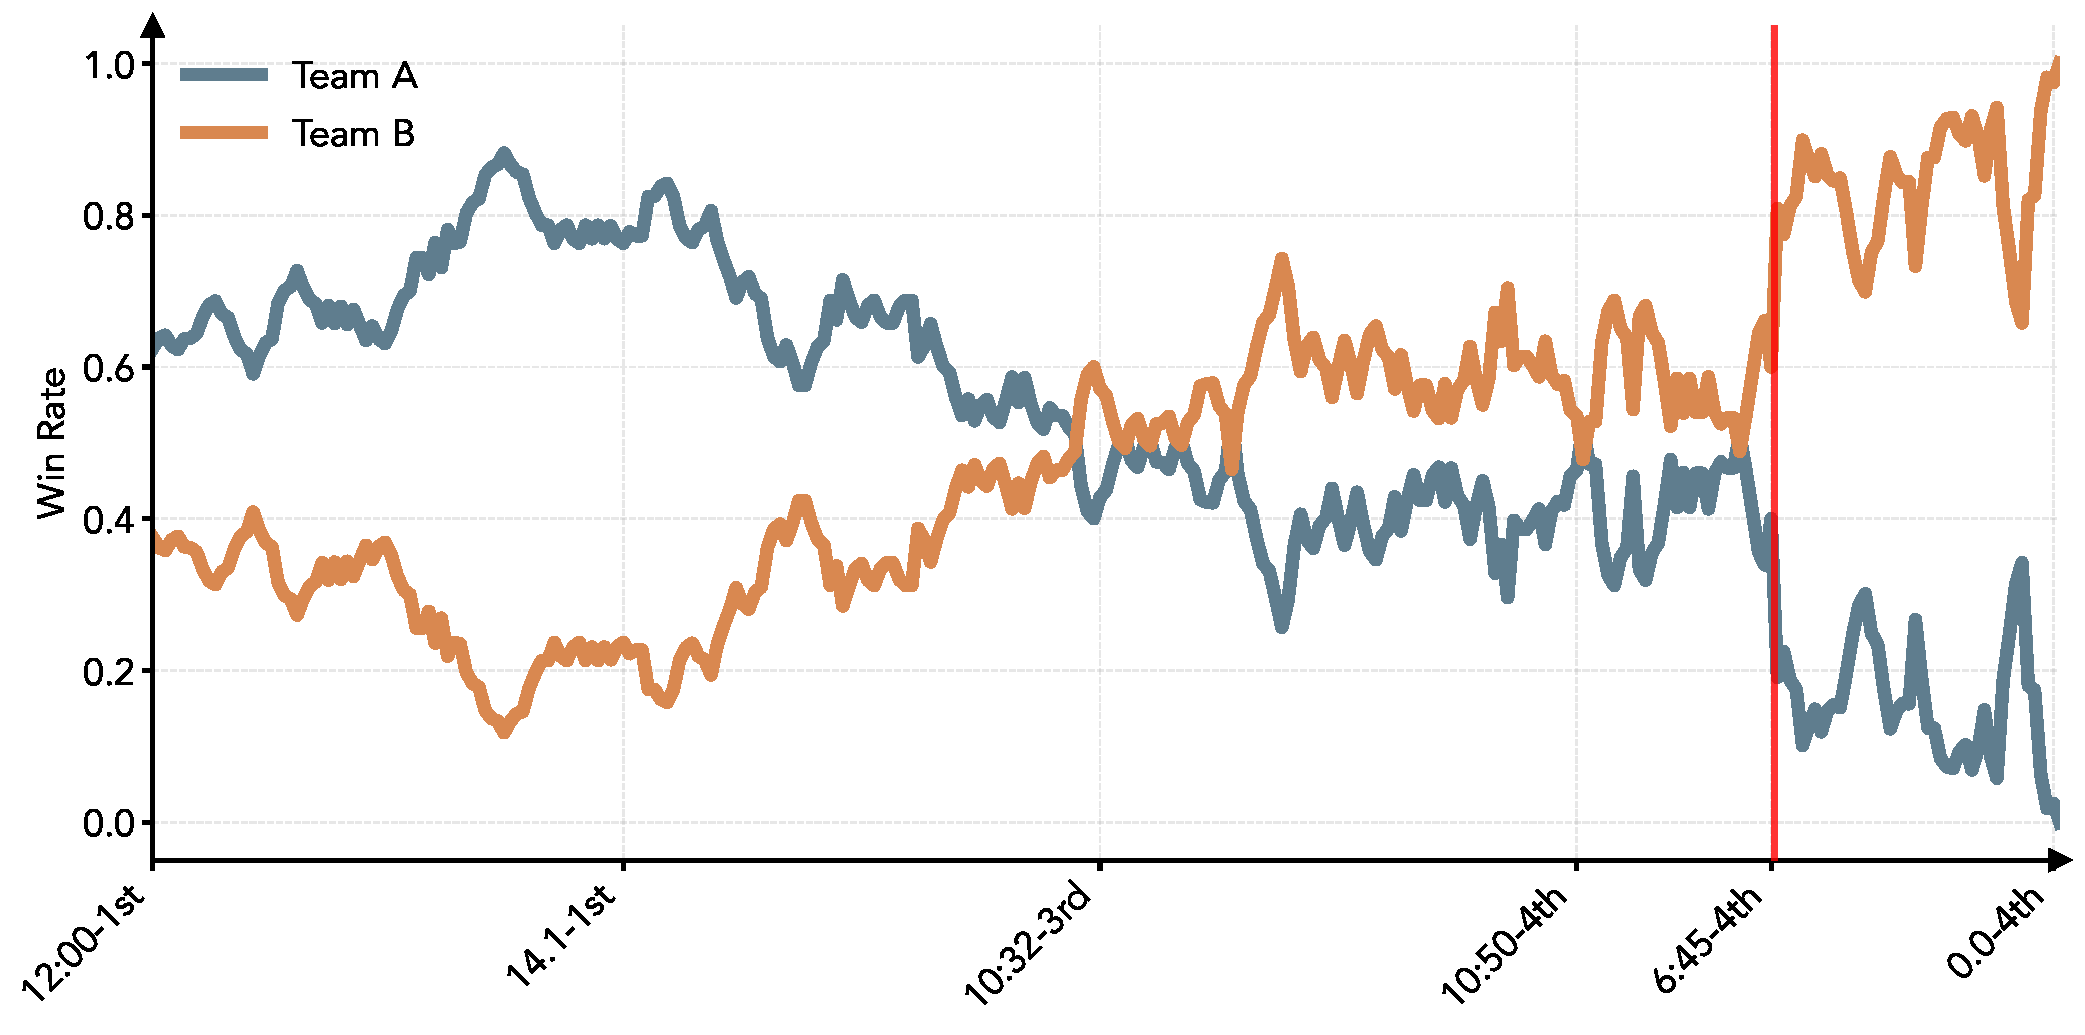
\includegraphics[width=\linewidth]{blocks/sample_cases_success/team_win_rate_series.pdf}
        % 调整底部的留白
        \vspace{-20pt}
    \end{wrapfigure}
        \textbf{Question:} You are an expert in basketball game analysis. Given a sequence of past events, future events, and corresponding time series data from a game, determine the most plausible event that occurred in between to link them.
        
        \textbf{Past Events:} \\
        12:00-1st: Player 6 (Team A) vs. Player 3 (Team B) (Player 2 (Team B) gains possession)\\
        11:38-1st: Player 6 (Team B) misses 27-foot three-point jumper\\
        \ldots \\
        6:56-4th: Player 6 (Team B) makes 25-foot three-point jumper (Player 7 (Team B) assists) | Team A Full timeout | Player 2 (Team A) enters the game for Player 9 (Team A) | Player 6 (Team A) enters the game for Player 7 (Team A)\\
        
        % \vspace{0.2cm}
        6:45-4th: [A CRITICAL EVENT HAPPENED HERE]\\ 
        % \vspace{0.2cm}
        \textbf{Future Events:} \\
        6:39-4th: Player 6 (Team A) offensive rebound \\
        6:33-4th: Player 2 (Team A) misses 27-foot step back jumpshot \\
        \ldots \\
        0:0-4th: End of the 4th Quarter | End of Game \\
        
        \vspace{0.2cm}
        \textbf{--- TASK ---} \\
        Based on the game's context and the data provided up to this point, what was the most likely event to occur? \\
        \textbf{Answer Choices}: (A) Player 3 (Team A) misses 20-foot two point shot \\ (B) Player 3 (Team A) misses driving floating jump shot \\  (C) Player 13 (Team A) blocks Player 19 (Team B) 's 5-foot two point shot \\ (D) Player 3 (Team A) makes 13-foot jumper (Player 6 (Team A) assists)\\
        \textbf{Correct Answer:} \textcolor{correctgreen}{(B)} \\
        \vspace{0.2cm}

    \vspace{0.5em}
\end{ReasoningBox}